\section{AIIDE: Artificial Intelligence and Interactive Digital Entertainment}\label{subsecAIIDE}

The AIIDE Starcraft AI Competition is the longest running annual Starcraft competition, and has been held every year since 2010 along with the AAAI Artificial Intelligence and Interactive Digital Entertainment conference. Unlike the CIG and SSCAIT competitions, the AIIDE competition requires (since 2011) that all bots be open source, and that their source code will be published for public download after the competition has finished. Running 24 hours a day for 2 weeks with games played at super-human speed, the competition is a single round-robin format with the winner being the bot with the highest win percentage when the time limit has been reached. 

\subsection{AIIDE 2010 - The First StarCraft AI Competition}

The AIIDE Starcraft AI Competition was first run in 2010 by Ben Weber at the Expressive Intelligence Studio at University of California, Santa Cruz, as part of the AIIDE (Artificial Intelligence and Interactive Digital Entertainment) conference. A total of 26 entrants competed in four different game modes which varied from simple combat battles to the full game of Starcraft. As this was the first year of the competition, and little infrastructure had been created, each game of the tournament was run manually on two laptop computers and monitored by hand to record the results. Also, no persistent data was kept for bots to learn about opponents between matches. The 2010 competition had 4 different tournament categories in which to compete. Tournament 1 was a flat-terrain unit micro-management battle consisting of four separate unit composition games. Of the six competitors, FreSCBot won the competition with Sherbrooke coming in 2nd place. Tournament 2 was another micro-focused game with non-trivial terrain. Two competitors submitted for this category, with FreSCBot once again coming in 1st by beating Sherbrooke. Tournament 3 was a tech-limited StarCraft game on a single known map with no fog-of-war enforced. Players were only allowed to choose the Protoss race, with no late game units allowed. 8 bots faced off in this double-elimination tournament with MimicBot taking first place over Botnik in the final. As this was a perfect information variant of StarCraft, MimicBot adopted a strategy of ``mimic its opponent's build order, gaining an economic advantage whenever possible'' which worked quite well.

Tournament 4 was considered the main event, which involved playing the complete game of StarCraft: Brood War with fog-of-war enforced. The tournament was run with a random pairing double-elimination format with each match being best of 5 games. Competitors could play as any of the three races, with the only limitations in gameplay being those that were considered ``cheating'' in the StarCraft community. Since computer programs written with BWAPI have no limit to the number of actions they can issue to the Starcraft game engine, certain behaviours are possible which were not intended by the developers such as sliding buildings and walking ground units over walls, these sorts of actions are considered cheating and not allowed in the tournament. A map pool of 5 well-known professional maps were announced to competitors in advance, with a random map being chosen for each game. Tournament 4 was won by Overmind - a Zerg bot created by a large team from the University of California, Berkeley, who defeated the Terran bot Krasi0 by Krasimir Krastev in the finals.

Overmind relied heavily on using the powerful and agile Zerg Mutalisk flying unit, which it controlled to great success using potential fields. Overmind's overall strategy consisted of an initial defense of Zerglings and Sunken Colonies (static defense towers) to protect its initial expansion while gathering enough resources to construct its initial Mutalisks. Once the Mutalisks had been constructed, it sent them to the enemy base and patrolled and harasses around the perimiter of the enemy base. If the bot did not win outright on the initial attack, it would slowly patrol and pick off any units which were undefended, eventually wearing down the enemy to the point where it could overwhelm it with a final attack. The 2nd place bot krasi0 played a very defensive Terran strategy, constructing Bunkers, Sige Tanks, and Missle Turrets for defense. After a certain number of units had been constructed it would then send an army of mechanical units to siege the enemy base. This bot performed quite well, only losing to Overmind during the competition. An excellent article about Overmind was written by Ars Technica in 2011.

\subsection{2011 - Automated Game Playing}
From 2011 to 2016, the AIIDE competition was hosted by the University of Alberta, and was organized and run each year by David Churchill and Michael Buro. Due to the low number of entries to Tournaments 1, 2, and 3 from the 2010 AIIDE competition, it was decided that the AIIDE competition for 2011 would only consist of the full game of Starcraft (with the same rules as the 2010 Tournament 4), with no smaller micromanagement tournaments. The 2011 tournament rules were also updated so that all entrants must submit the source code of their bot and allow it to be published after the competition is over, which was done for a few reasons. One reason was to lower the barrier to entry for future competitions - since programming a Starcraft AI bot was very time consuming, future entrants could download and modify the source code of previous bots to save considerable effort. Another reason was to more easily prevent cheating - with thousands of games being played in the tournament we could no longer watch each game to detect if any cheating tactics were being employed, which would be more easily detected by inspecting the source code (which was not allowed to be heavily obfuscated). The final reason was to help advance the state of the art in Starcraft AI by allowing future bots to borrow strategies and techniques of previous bots by inspecting their source code - ideally, all bots in future competitions should be at least as strong as the bots from the previous year. The 2011 competition received 13 entrants. 

The 2010 tournament was run Ben Weber on two laptops, and games were played by manually starting the Starcraft game and creating and joining games by hand. As the physical demand was quite high, a simple random-pairing double-elimination tournament was played with approximately 60 games in total. This caused some negative feedback that results this elimination-style tournament was quite dependent on pairing luck, so for the 2011 competition we set out to eliminate all randomness from the tournament and play a round robin style format. Playing a round robin format requires far more games to be played, and would no longer be possible to run each game manually. In the summer of 2011, David Churchill, Jason Lorenz, and Michael Buro wrote the StarCraft AI Tournament Managing software (see section X) which could automatically schedule and play a round robin tournaments of Starcraft on an arbitrary number of locally networked computers. This software used a server/client architecture with a single server machine scheduling games and storing results, and each other machine running the client software which started the Starcraft game, monitored the game's progress and recorded the results when finished. Bot files, replays, and final results were accessed by clients via a shared Windows folder on the local network which was visible to all client machines. The initial version of this software allowed for a total of 2340 games to be played in the same time period as the 2010 competition's 60 games, with each bot playing each other bot a total of 30 times. There were 10 total maps in the competition, chosen from expert human tournaments that were known to be balanced for each race, and were available for download several months in advance on the competition website. The AIIDE competition was modeled on human tournaments where the map pool and opponents are known in advance in order to allow for some expert knowledge and opponent modeling.

At the end of the five day competition, Skynet placed 1st, UAlbertaBot placed 2nd, and Aiur placed 3rd. Skynet is a Protoss bot written by Andrew Smith, a software engineer from the United Kingdom, and used a number of solid Protoss strategies such as a Zealot rush, Dragoon / Zealot mid-game army, and a late game army consisting of Zealots, Dragoons, and Reavers. Its soloid economic play and good early defense were able to hold off the more offensive Protoss bots of UAlbertaBot and Aiur.

\subsection{AIIDE 2016-17 Updates \& News}\label{subsecAIIDEnews}

The 2016 AIIDE competition had a total of 21 competitors, and the round robin games ran on 12 machines for nearly two weeks. A total of 90 round robin rounds were completed, with each bot playing 1800 games. No new rules or maps were used for the 2016 tournament that were not in place for the 2015 tournament. As the AIIDE competition was held shortly after the CIG competition, many of the submissions were the same, which is reflected in the results of both competitions. The top four finishers can be seen in Figure \ref{figAIIDEresults}, with Iron placing 1st, ZZZKbot placing 2nd, and tscmoo coming in 3rd place.

\vskip 2mm
\begin{figure}[h]
  \centering
  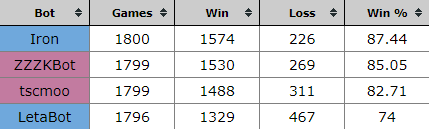
\includegraphics[width=1\columnwidth]{fig/aiide2016.png}
  \caption{Results of the top 4 finishers in the 2016 AIIDE competition. Iron and LetaBot are Terran bots, while ZZZBot and tscmoo played as Zerg.}
  \label{figAIIDEresults}
\end{figure}

In 2016, the AIIDE competition website was updated to include an archive\footnote{\url{http://www.cs.mun.ca/~dchurchill/starcraftaicomp/archive.shtml}} of data and results of all of the annual AIIDE and CIG competitions, including final results, bot source code and binary download links, and information about each bot. 

The 2017 AIIDE competition will have several updates:

\begin{itemize}
\item An updated map pool consisting of 10 new maps.
\item Updated tournament managing software capable of playing more games in the same period of time.
\item Support for BWAPI version 4.2.0
\item Bots that achieved a 30\% or higher win rate in the 2016 competition will be carried forward to 2017
\item Plans to support GPU computation for bots
\end{itemize}

\vskip 6mm